% Options for packages loaded elsewhere
\PassOptionsToPackage{unicode}{hyperref}
\PassOptionsToPackage{hyphens}{url}
%
\documentclass[
]{article}
\usepackage{amsmath,amssymb}
\usepackage{iftex}
\ifPDFTeX
  \usepackage[T1]{fontenc}
  \usepackage[utf8]{inputenc}
  \usepackage{textcomp} % provide euro and other symbols
\else % if luatex or xetex
  \usepackage{unicode-math} % this also loads fontspec
  \defaultfontfeatures{Scale=MatchLowercase}
  \defaultfontfeatures[\rmfamily]{Ligatures=TeX,Scale=1}
\fi
\usepackage{lmodern}
\ifPDFTeX\else
  % xetex/luatex font selection
\fi
% Use upquote if available, for straight quotes in verbatim environments
\IfFileExists{upquote.sty}{\usepackage{upquote}}{}
\IfFileExists{microtype.sty}{% use microtype if available
  \usepackage[]{microtype}
  \UseMicrotypeSet[protrusion]{basicmath} % disable protrusion for tt fonts
}{}
\makeatletter
\@ifundefined{KOMAClassName}{% if non-KOMA class
  \IfFileExists{parskip.sty}{%
    \usepackage{parskip}
  }{% else
    \setlength{\parindent}{0pt}
    \setlength{\parskip}{6pt plus 2pt minus 1pt}}
}{% if KOMA class
  \KOMAoptions{parskip=half}}
\makeatother
\usepackage{xcolor}
\usepackage[margin=1in]{geometry}
\usepackage{longtable,booktabs,array}
\usepackage{calc} % for calculating minipage widths
% Correct order of tables after \paragraph or \subparagraph
\usepackage{etoolbox}
\makeatletter
\patchcmd\longtable{\par}{\if@noskipsec\mbox{}\fi\par}{}{}
\makeatother
% Allow footnotes in longtable head/foot
\IfFileExists{footnotehyper.sty}{\usepackage{footnotehyper}}{\usepackage{footnote}}
\makesavenoteenv{longtable}
\usepackage{graphicx}
\makeatletter
\def\maxwidth{\ifdim\Gin@nat@width>\linewidth\linewidth\else\Gin@nat@width\fi}
\def\maxheight{\ifdim\Gin@nat@height>\textheight\textheight\else\Gin@nat@height\fi}
\makeatother
% Scale images if necessary, so that they will not overflow the page
% margins by default, and it is still possible to overwrite the defaults
% using explicit options in \includegraphics[width, height, ...]{}
\setkeys{Gin}{width=\maxwidth,height=\maxheight,keepaspectratio}
% Set default figure placement to htbp
\makeatletter
\def\fps@figure{htbp}
\makeatother
\setlength{\emergencystretch}{3em} % prevent overfull lines
\providecommand{\tightlist}{%
  \setlength{\itemsep}{0pt}\setlength{\parskip}{0pt}}
\setcounter{secnumdepth}{-\maxdimen} % remove section numbering
\ifLuaTeX
  \usepackage{selnolig}  % disable illegal ligatures
\fi
\usepackage{bookmark}
\IfFileExists{xurl.sty}{\usepackage{xurl}}{} % add URL line breaks if available
\urlstyle{same}
\hypersetup{
  pdftitle={Data Science 2 Midterm},
  hidelinks,
  pdfcreator={LaTeX via pandoc}}

\title{Data Science 2 Midterm}
\author{}
\date{\vspace{-2.5em}}

\begin{document}
\maketitle

\section{Exploratory Analysis}\label{exploratory-analysis}

For datasets \textbf{dat1} and \textbf{dat2} initial exploration of the
data structure, descriptive statistics of continuous variables,
correlation analysis, and various visualization techniques were
conducted.

\textless\textless\textless\textless\textless\textless\textless{} HEAD
Looking at \textbf{dat1}, the distribution of \textbf{$log_antibody$} is
approximately normal, as seen in Figure @ref(fig:d1-log-antibody-hist)
and Figure @ref(fig:d1-log-antibody-qq). High and low outliers can be
observed in the Figure @ref(fig:d1-log-antibody-box). Most covariates
have weak or low correlation with each other. There is a high positive
correlation between \textbf{bmi} and \textbf{weight} (\(\rho = 0.72\))
and a moderate negative correlation between \textbf{bmi} and
\textbf{height} (\(\rho = -0.50\)). There is a mild negative correlation
between \textbf{$log_antibody$} and \textbf{bmi} (\(\rho = -0.23\)),
\textbf{weight} (\(\rho = -0.17\)), and \textbf{age} (\(\rho = -0.15\)).
There is a mild positive correlation between \textbf{$log_antibody$} and
\textbf{height} (\(\rho = 0.10\)). The correlation between
\textbf{$log_antibody$} and \textbf{SBP} (\(\rho = -0.06\)),
\textbf{LDL} (\(\rho = -0.04\)), and \textbf{time} (\(\rho = -0.01\))
are near zero, indicating no linear relationship. Linear relationships
can be seen in Figure

\section{\texorpdfstring{Exploring \textbf{dat2}, the distribution of
\textbf{$log_antibody$} is also approximately normal, as shown Figure
@ref(fig:d2-log-antibody-hist) and Figure @ref(fig:d2-log-antibody-qq).
High and low outliers are again visible in the Figure
@ref(fig:d2-log-antibody-box). Most covariates exhibit weak or low
correlation with each other. There is a high positive correlation
between \textbf{bmi} and \textbf{weight} (\(\rho = 0.72\)) and a
moderate negative correlation between \textbf{bmi} and \textbf{height}
(\(\rho = -0.53\)). There is a mild negative correlation between
\textbf{log_antibody} and \textbf{bmi} (\(\rho = -0.16\)),
\textbf{weight} (\(\rho = -0.11\)), and \textbf{age} (\(\rho = -0.08\)).
A mild positive correlation exists between \textbf{$log_antibody$} and
\textbf{height} (\(\rho = 0.08\)). The correlations between
\textbf{$log_antibody$} and \textbf{SBP} (\(\rho = -0.01\)),
\textbf{LDL} (\(\rho = -0.00\)), and \textbf{time} (\(\rho = -0.25\))
are near zero or weak, again suggesting no strong linear relationship.
Linear relationships can be seen in
Figure}{Exploring , the distribution of  is also approximately normal, as shown Figure @ref(fig:d2-log-antibody-hist) and Figure @ref(fig:d2-log-antibody-qq). High and low outliers are again visible in the Figure @ref(fig:d2-log-antibody-box). Most covariates exhibit weak or low correlation with each other. There is a high positive correlation between  and  (\textbackslash rho = 0.72) and a moderate negative correlation between  and  (\textbackslash rho = -0.53). There is a mild negative correlation between  and  (\textbackslash rho = -0.16),  (\textbackslash rho = -0.11), and  (\textbackslash rho = -0.08). A mild positive correlation exists between  and  (\textbackslash rho = 0.08). The correlations between  and  (\textbackslash rho = -0.01),  (\textbackslash rho = -0.00), and  (\textbackslash rho = -0.25) are near zero or weak, again suggesting no strong linear relationship. Linear relationships can be seen in Figure}}\label{exploring-the-distribution-of-is-also-approximately-normal-as-shown-figure-reffigd2-log-antibody-hist-and-figure-reffigd2-log-antibody-qq.-high-and-low-outliers-are-again-visible-in-the-figure-reffigd2-log-antibody-box.-most-covariates-exhibit-weak-or-low-correlation-with-each-other.-there-is-a-high-positive-correlation-between-and-rho-0.72-and-a-moderate-negative-correlation-between-and-rho--0.53.-there-is-a-mild-negative-correlation-between-and-rho--0.16-rho--0.11-and-rho--0.08.-a-mild-positive-correlation-exists-between-and-rho-0.08.-the-correlations-between-and-rho--0.01-rho--0.00-and-rho--0.25-are-near-zero-or-weak-again-suggesting-no-strong-linear-relationship.-linear-relationships-can-be-seen-in-figure}

Looking at \textbf{dat1}, the distribution of \textbf{log\_antibody} is
approximately normal, as seen in Figure @ref(fig:d1-log-antibody-hist)
and Figure @ref(fig:d1-log-antibody-qq). High and low outliers can be
observed in the Figure \ref{fig:d1-log-antibody-box}. Most covariates
have weak or low correlation with each other. There is a high positive
correlation between \textbf{bmi} and \textbf{weight} (\(\rho = 0.72\))
and a moderate negative correlation between \textbf{bmi} and
\textbf{height} (\(\rho = -0.50\)). There is a mild negative correlation
between \textbf{log\_antibody} and \textbf{bmi} (\(\rho = -0.23\)),
\textbf{weight} (\(\rho = -0.17\)), and \textbf{age} (\(\rho = -0.15\)).
There is a mild positive correlation between \textbf{log\_antibody} and
\textbf{height} (\(\rho = 0.10\)). The correlation between
\textbf{log\_antibody} and \textbf{SBP} (\(\rho = -0.06\)), \textbf{LDL}
(\(\rho = -0.04\)), and \textbf{time} (\(\rho = -0.01\)) are near zero,
indicating no linear relationship. Linear relationships can be seen in
Figure

Exploring \textbf{dat2}, the distribution of \textbf{log\_antibody} is
also approximately normal, as shown Figure
@ref(fig:d2-log-antibody-hist) and Figure @ref(fig:d2-log-antibody-qq).
High and low outliers are again visible in the Figure
@ref(fig:d2-log-antibody-box). Most covariates exhibit weak or low
correlation with each other. There is a high positive correlation
between \textbf{bmi} and \textbf{weight} (\(\rho = 0.72\)) and a
moderate negative correlation between \textbf{bmi\} and }height\}
(\(\rho = -0.53\)). There is a mild negative correlation between
\textbf{log\_antibody} and \textbf{bmi} (\(\rho = -0.16\)),
\textbf{weight} (\(\rho = -0.11\)), and \textbf{age} (\(\rho = -0.08\)).
A mild positive correlation exists between \textbf{log\_antibody} and
\textbf{height} (\(\rho = 0.084\)). The correlations between
\textbf{log\_antibody} and \textbf{SBP} (\(\rho = -0.01\)), \textbf{LDL}
(\(\rho = -0.00\)), and \textbf{time} (\(\rho = -0.25\)) are near zero
or weak, again suggesting no strong linear relationship. Linear
relationships can be seen in Figure
\textgreater\textgreater\textgreater\textgreater\textgreater\textgreater\textgreater{}
f5e371ff37c9e841cbcaba1343c15e0de86916ee

\begin{verbatim}
## Warning: Expected 2 pieces. Additional pieces discarded in 6 rows [67, 68, 69, 70, 71,
## 72].
\end{verbatim}

\begin{longtable}[]{@{}
  >{\raggedright\arraybackslash}p{(\columnwidth - 12\tabcolsep) * \real{0.1625}}
  >{\raggedleft\arraybackslash}p{(\columnwidth - 12\tabcolsep) * \real{0.1375}}
  >{\raggedleft\arraybackslash}p{(\columnwidth - 12\tabcolsep) * \real{0.1500}}
  >{\raggedleft\arraybackslash}p{(\columnwidth - 12\tabcolsep) * \real{0.1375}}
  >{\raggedleft\arraybackslash}p{(\columnwidth - 12\tabcolsep) * \real{0.1375}}
  >{\raggedleft\arraybackslash}p{(\columnwidth - 12\tabcolsep) * \real{0.1375}}
  >{\raggedleft\arraybackslash}p{(\columnwidth - 12\tabcolsep) * \real{0.1375}}@{}}
\caption{Clean Summary Statistics for Numeric Variables}\tabularnewline
\toprule\noalign{}
\begin{minipage}[b]{\linewidth}\raggedright
Variable
\end{minipage} & \begin{minipage}[b]{\linewidth}\raggedleft
Min
\end{minipage} & \begin{minipage}[b]{\linewidth}\raggedleft
Q1
\end{minipage} & \begin{minipage}[b]{\linewidth}\raggedleft
Median
\end{minipage} & \begin{minipage}[b]{\linewidth}\raggedleft
Mean
\end{minipage} & \begin{minipage}[b]{\linewidth}\raggedleft
Q3
\end{minipage} & \begin{minipage}[b]{\linewidth}\raggedleft
Max
\end{minipage} \\
\midrule\noalign{}
\endfirsthead
\toprule\noalign{}
\begin{minipage}[b]{\linewidth}\raggedright
Variable
\end{minipage} & \begin{minipage}[b]{\linewidth}\raggedleft
Min
\end{minipage} & \begin{minipage}[b]{\linewidth}\raggedleft
Q1
\end{minipage} & \begin{minipage}[b]{\linewidth}\raggedleft
Median
\end{minipage} & \begin{minipage}[b]{\linewidth}\raggedleft
Mean
\end{minipage} & \begin{minipage}[b]{\linewidth}\raggedleft
Q3
\end{minipage} & \begin{minipage}[b]{\linewidth}\raggedleft
Max
\end{minipage} \\
\midrule\noalign{}
\endhead
\bottomrule\noalign{}
\endlastfoot
id & 1.000000 & 1250.750000 & 2500.50000 & 2500.50000 & 3750.25000 &
5000.00000 \\
age & 44.000000 & 57.000000 & 60.00000 & 59.96840 & 63.00000 &
75.00000 \\
gender & 0.000000 & 0.000000 & 0.00000 & 0.48540 & 1.00000 & 1.00000 \\
height & 150.200000 & 166.100000 & 170.10000 & 170.12634 & 174.22500 &
192.90000 \\
weight & 56.700000 & 75.400000 & 80.10000 & 80.10908 & 84.90000 &
106.00000 \\
bmi & 18.200000 & 25.800000 & 27.60000 & 27.74040 & 29.50000 &
38.80000 \\
diabetes & 0.000000 & 0.000000 & 0.00000 & 0.15440 & 0.00000 &
1.00000 \\
hypertension & 0.000000 & 0.000000 & 0.00000 & 0.45960 & 1.00000 &
1.00000 \\
SBP & 101.000000 & 124.000000 & 130.00000 & 129.90040 & 135.00000 &
155.00000 \\
LDL & 43.000000 & 96.000000 & 110.00000 & 109.90860 & 124.00000 &
185.00000 \\
time & 30.000000 & 76.000000 & 106.00000 & 108.86260 & 138.00000 &
270.00000 \\
log & 7.765405 & 9.681635 & 10.08908 & 10.06434 & 10.47758 & 11.96137 \\
\end{longtable}

\begin{figure}

{\centering 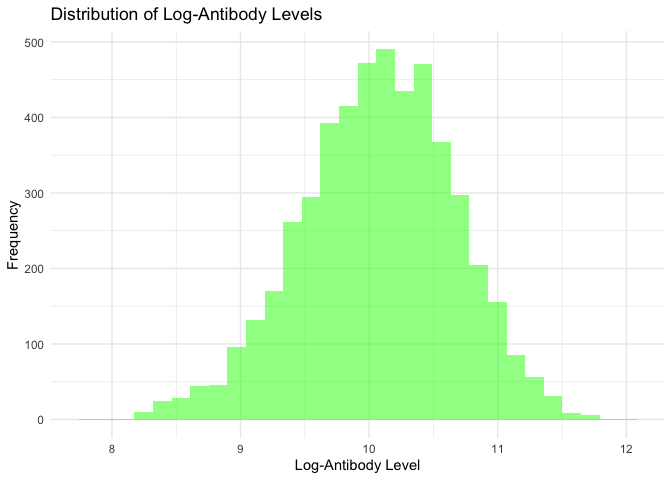
\includegraphics[width=0.33\linewidth]{DS2_Midterm_files/figure-latex/d1-log-antibody-hist-1} 

}

\caption{Histogram of log\_antibody levels for dat1}\label{fig:d1-log-antibody-hist}
\end{figure}

\begin{figure}

{\centering 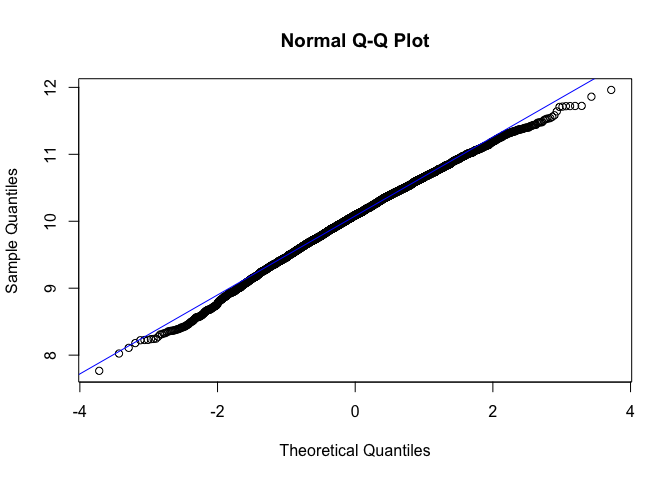
\includegraphics[width=0.33\linewidth]{DS2_Midterm_files/figure-latex/d1-log-antibody-qq-1} 

}

\caption{Q-Q plot of log\_antibody levels for dat1}\label{fig:d1-log-antibody-qq}
\end{figure}

\begin{figure}

{\centering 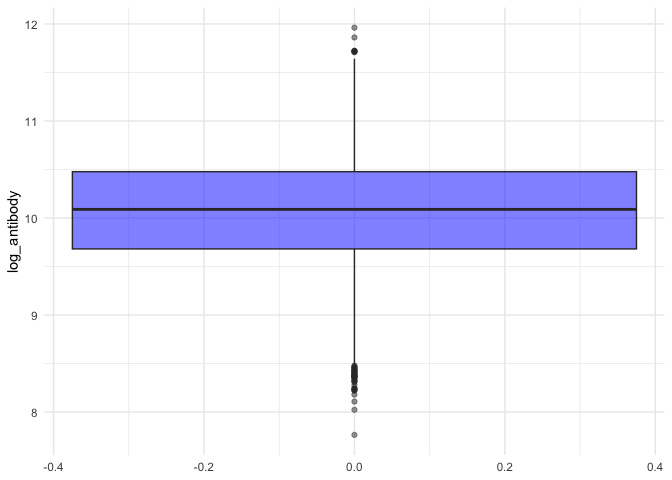
\includegraphics[width=0.33\linewidth]{DS2_Midterm_files/figure-latex/d1-log-antibody-box-1} 

}

\caption{Boxplot of log\_antibody levels for dat1}\label{fig:d1-log-antibody-box}
\end{figure}

\begin{figure}
\centering
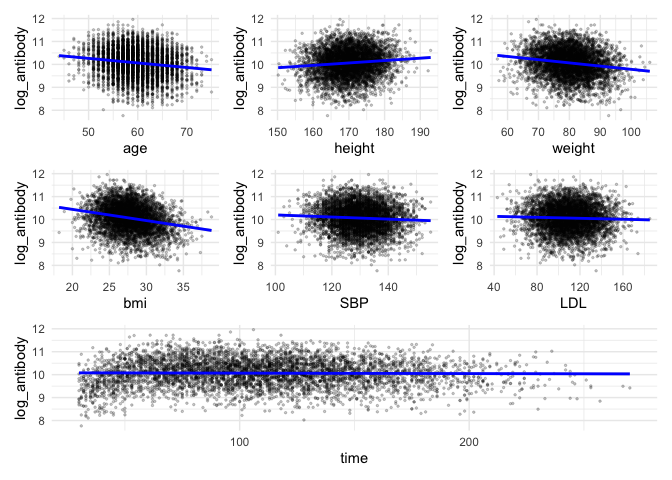
\includegraphics{DS2_Midterm_files/figure-latex/d1-log-antibody-lin-1.pdf}
\caption{Linearity between log\_antibody levels and covariates for dat1}
\end{figure}

\begin{figure}

{\centering 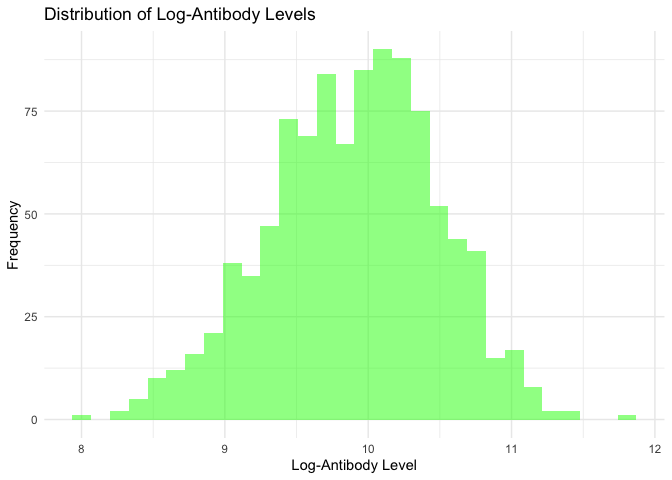
\includegraphics[width=0.33\linewidth]{DS2_Midterm_files/figure-latex/d2-log-antibody-hist-1} 

}

\caption{Histogram of log\_antibody levels for dat2}\label{fig:d2-log-antibody-hist}
\end{figure}

\begin{figure}

{\centering 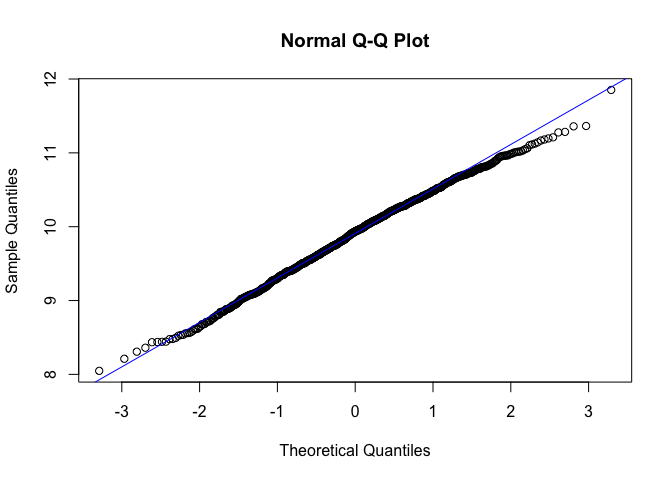
\includegraphics[width=0.33\linewidth]{DS2_Midterm_files/figure-latex/d2-log-antibody-qq-1} 

}

\caption{Q-Q plot of log\_antibody levels for dat2}\label{fig:d2-log-antibody-qq}
\end{figure}

\begin{figure}

{\centering 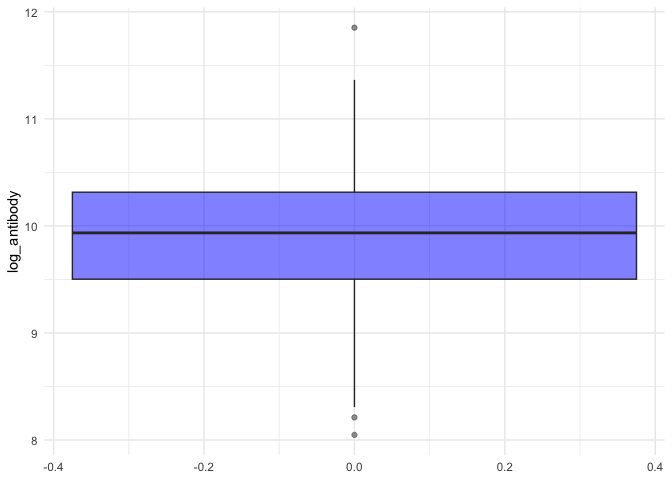
\includegraphics[width=0.33\linewidth]{DS2_Midterm_files/figure-latex/d2-log-antibody-box-1} 

}

\caption{Boxplot of log\_antibody levels for dat2}\label{fig:d2-log-antibody-box}
\end{figure}

\begin{figure}
\centering
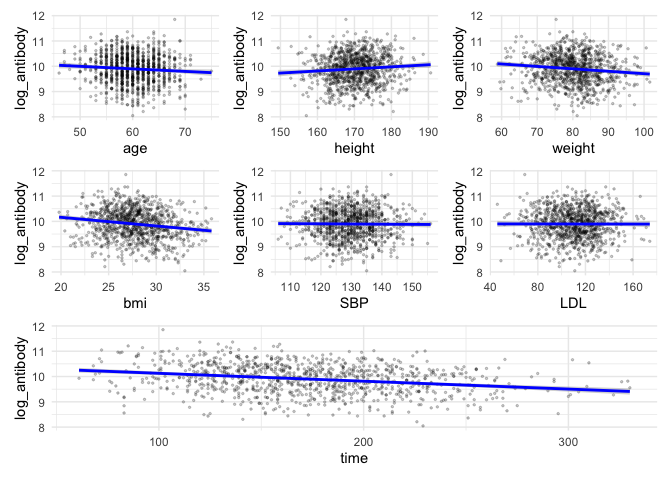
\includegraphics{DS2_Midterm_files/figure-latex/d2-log-antibody-lin-1.pdf}
\caption{Linearity between log\_antibody levels and covariates for dat2}
\end{figure}

\begin{center}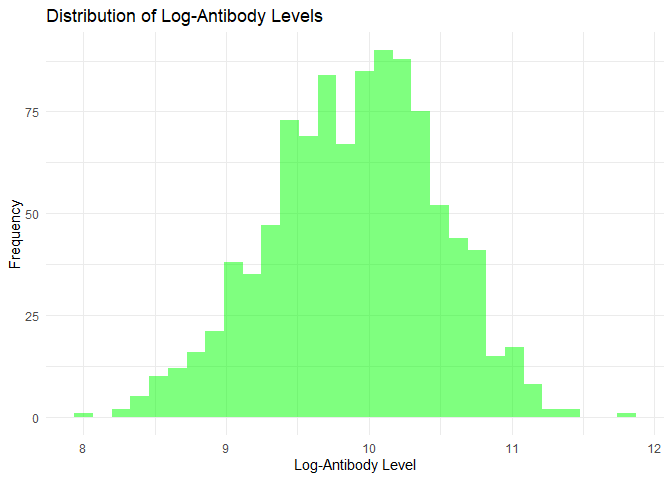
\includegraphics[width=0.8\linewidth]{DS2_Midterm_files/figure-latex/unnamed-chunk-14-1} \end{center}

\begin{center}\includegraphics[width=0.8\linewidth]{DS2_Midterm_files/figure-latex/unnamed-chunk-14-2} \end{center}

\begin{center}\includegraphics[width=0.8\linewidth]{DS2_Midterm_files/figure-latex/unnamed-chunk-14-3} \end{center}

The exploration and evaluation of \textbf{dat1} is used to help build a
prediction model specific ally using GAM to understand how demographic
and clinical factors influence antibody responses and how antibody
levels change over time following vaccination. Considering the
researcher collects a new and independent dataset, \textbf{dat2}, we
discover the correlation between \textbf{time} and
\textbf{log\_antibody} is stronger than in \textbf{dat1} and similarly
has weak linear relationships with most covariates. \textbf{Dat2} allows
us to evaluate the robustness and generalizability of our prediction
model.

\section{Model Trainging}\label{model-trainging}

A Generalized Additive Model (GAM) was created to model log-transformed
antibody level. Predictors included age, gender, race, smoking, height,
weight, BMI, diabetes, hypertension, SBP, LDL, and time since
vaccination. To prepare the data for modeling, the model matrix, x, was
created using the outcome and all predictors listed above and extracted
the response variable, y. Given that race and smoking were categorical
variables with multiple categories, some re-coding was necessary to use
these variables in the model building. Therefore, race and smoking were
converted into factor variables with ``White'' being the reference group
for race and ``Never'' being the reference group for smoking.

The GAM models were then fitted. The first model, gam.m1, is a standard
linear model with no smoothing terms. The second model, gam.m2, uses
smoothing on age, bmi, SBP, LDL, and time since vaccination. There was
reason to believe these variables were non-linear, therefore the
smoothing allowed the variables to be used in the model. Finally, model
3, gam.m3, includes a tensor product to model the interaction between
height and weight.

The three GAM models were then compared using an ANOVA test that
provides the f-test; this was used to determine which model provides the
best fit. Cross-validation for GAM tuning was then conducted using a
10-fold cross-validation to tune to GAM model. The best hyperparameters
and the final fitted model were then retrieved. The same model training
procedure was used with the new, independent dataset, dat2.

\begin{longtable}[]{@{}
  >{\raggedright\arraybackslash}p{(\columnwidth - 12\tabcolsep) * \real{0.1045}}
  >{\raggedleft\arraybackslash}p{(\columnwidth - 12\tabcolsep) * \real{0.1493}}
  >{\raggedleft\arraybackslash}p{(\columnwidth - 12\tabcolsep) * \real{0.1642}}
  >{\raggedleft\arraybackslash}p{(\columnwidth - 12\tabcolsep) * \real{0.1343}}
  >{\raggedleft\arraybackslash}p{(\columnwidth - 12\tabcolsep) * \real{0.1642}}
  >{\raggedleft\arraybackslash}p{(\columnwidth - 12\tabcolsep) * \real{0.1343}}
  >{\raggedleft\arraybackslash}p{(\columnwidth - 12\tabcolsep) * \real{0.1493}}@{}}
\caption{ANOVA Comparison of GAM Models (Dat1)}\tabularnewline
\toprule\noalign{}
\begin{minipage}[b]{\linewidth}\raggedright
Model
\end{minipage} & \begin{minipage}[b]{\linewidth}\raggedleft
Resid. Df
\end{minipage} & \begin{minipage}[b]{\linewidth}\raggedleft
Resid. Dev
\end{minipage} & \begin{minipage}[b]{\linewidth}\raggedleft
Df
\end{minipage} & \begin{minipage}[b]{\linewidth}\raggedleft
Deviance
\end{minipage} & \begin{minipage}[b]{\linewidth}\raggedleft
F
\end{minipage} & \begin{minipage}[b]{\linewidth}\raggedleft
Pr(\textgreater F)
\end{minipage} \\
\midrule\noalign{}
\endfirsthead
\toprule\noalign{}
\begin{minipage}[b]{\linewidth}\raggedright
Model
\end{minipage} & \begin{minipage}[b]{\linewidth}\raggedleft
Resid. Df
\end{minipage} & \begin{minipage}[b]{\linewidth}\raggedleft
Resid. Dev
\end{minipage} & \begin{minipage}[b]{\linewidth}\raggedleft
Df
\end{minipage} & \begin{minipage}[b]{\linewidth}\raggedleft
Deviance
\end{minipage} & \begin{minipage}[b]{\linewidth}\raggedleft
F
\end{minipage} & \begin{minipage}[b]{\linewidth}\raggedleft
Pr(\textgreater F)
\end{minipage} \\
\midrule\noalign{}
\endhead
\bottomrule\noalign{}
\endlastfoot
gam.m1 & 4984.000 & 1509.442 & NA & NA & NA & NA \\
gam.m2 & 4971.177 & 1380.053 & 12.82350 & 129.389611 & 36.37749 &
0.0000000 \\
gam.m3 & 4968.540 & 1378.818 & 2.63652 & 1.234568 & 1.68820 &
0.1738572 \\
\end{longtable}

\begin{figure}
\centering
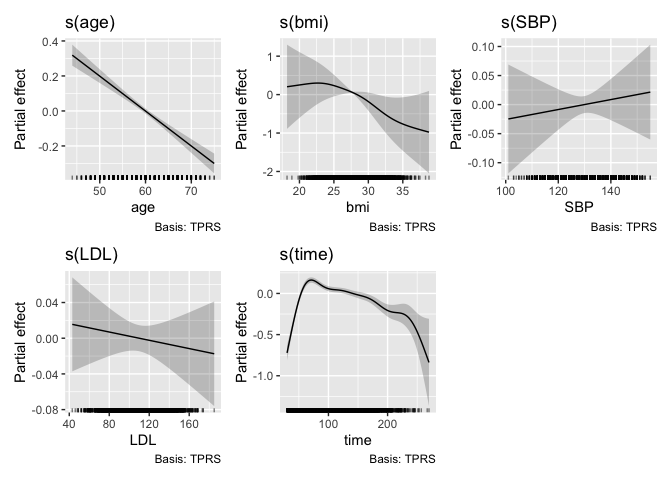
\includegraphics{DS2_Midterm_files/figure-latex/gam2-gridplot-1.pdf}
\caption{Smooth terms for GAM model (gam.m2)}
\end{figure}

\begin{figure}

{\centering 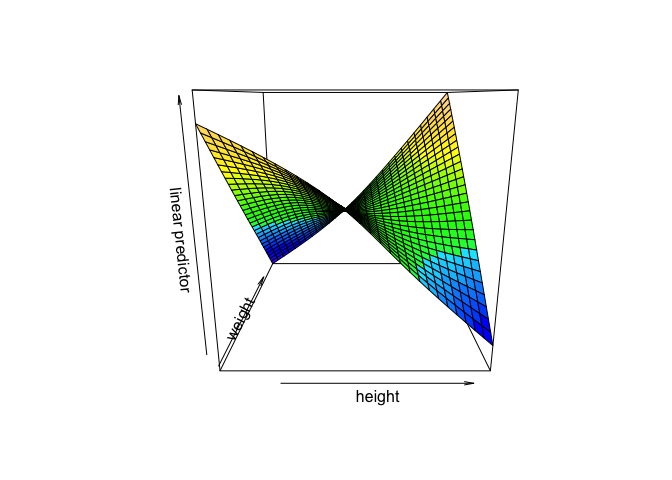
\includegraphics[width=0.9\linewidth]{DS2_Midterm_files/figure-latex/vis-gam-1} 

}

\caption{Visualization of Model 3 (dat1)}\label{fig:vis-gam}
\end{figure}

\begin{center}\includegraphics[width=0.8\linewidth]{DS2_Midterm_files/figure-latex/unnamed-chunk-17-1} \end{center}

\begin{center}\includegraphics[width=0.8\linewidth]{DS2_Midterm_files/figure-latex/unnamed-chunk-17-2} \end{center}

\begin{center}\includegraphics[width=0.8\linewidth]{DS2_Midterm_files/figure-latex/unnamed-chunk-17-3} \end{center}

\begin{longtable}[]{@{}
  >{\raggedright\arraybackslash}p{(\columnwidth - 12\tabcolsep) * \real{0.1045}}
  >{\raggedleft\arraybackslash}p{(\columnwidth - 12\tabcolsep) * \real{0.1493}}
  >{\raggedleft\arraybackslash}p{(\columnwidth - 12\tabcolsep) * \real{0.1642}}
  >{\raggedleft\arraybackslash}p{(\columnwidth - 12\tabcolsep) * \real{0.1343}}
  >{\raggedleft\arraybackslash}p{(\columnwidth - 12\tabcolsep) * \real{0.1493}}
  >{\raggedleft\arraybackslash}p{(\columnwidth - 12\tabcolsep) * \real{0.1493}}
  >{\raggedleft\arraybackslash}p{(\columnwidth - 12\tabcolsep) * \real{0.1493}}@{}}
\caption{ANOVA Comparison of GAM Models (Dat2)}\tabularnewline
\toprule\noalign{}
\begin{minipage}[b]{\linewidth}\raggedright
Model
\end{minipage} & \begin{minipage}[b]{\linewidth}\raggedleft
Resid. Df
\end{minipage} & \begin{minipage}[b]{\linewidth}\raggedleft
Resid. Dev
\end{minipage} & \begin{minipage}[b]{\linewidth}\raggedleft
Df
\end{minipage} & \begin{minipage}[b]{\linewidth}\raggedleft
Deviance
\end{minipage} & \begin{minipage}[b]{\linewidth}\raggedleft
F
\end{minipage} & \begin{minipage}[b]{\linewidth}\raggedleft
Pr(\textgreater F)
\end{minipage} \\
\midrule\noalign{}
\endfirsthead
\toprule\noalign{}
\begin{minipage}[b]{\linewidth}\raggedright
Model
\end{minipage} & \begin{minipage}[b]{\linewidth}\raggedleft
Resid. Df
\end{minipage} & \begin{minipage}[b]{\linewidth}\raggedleft
Resid. Dev
\end{minipage} & \begin{minipage}[b]{\linewidth}\raggedleft
Df
\end{minipage} & \begin{minipage}[b]{\linewidth}\raggedleft
Deviance
\end{minipage} & \begin{minipage}[b]{\linewidth}\raggedleft
F
\end{minipage} & \begin{minipage}[b]{\linewidth}\raggedleft
Pr(\textgreater F)
\end{minipage} \\
\midrule\noalign{}
\endhead
\bottomrule\noalign{}
\endlastfoot
gam.m1 & 984.0000 & 275.4546 & NA & NA & NA & NA \\
gam.m2 & 977.7820 & 268.5783 & 6.217997 & 6.8762407 & 4.0341782 &
0.0004416 \\
gam.m3 & 976.6323 & 268.2745 & 1.149679 & 0.3038207 & 0.9640406 &
0.3384056 \\
\end{longtable}

Model 2 (gam.m2) was chosen to be the final model based on the
improvements it made upon Model 1 (gam.m1), (pval=\textless0.001).

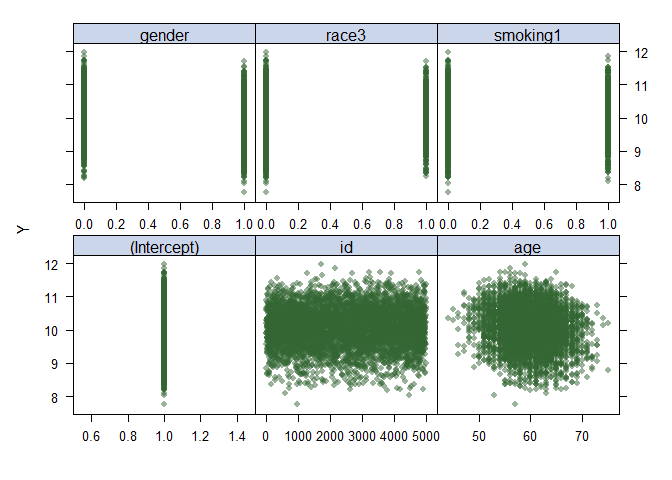
\includegraphics{DS2_Midterm_files/figure-latex/unnamed-chunk-19-1.pdf}

\begin{center}\includegraphics[width=0.9\linewidth]{DS2_Midterm_files/figure-latex/unnamed-chunk-20-1} \end{center}

\section{Final Model Results}\label{final-model-results}

\begin{figure}
\centering
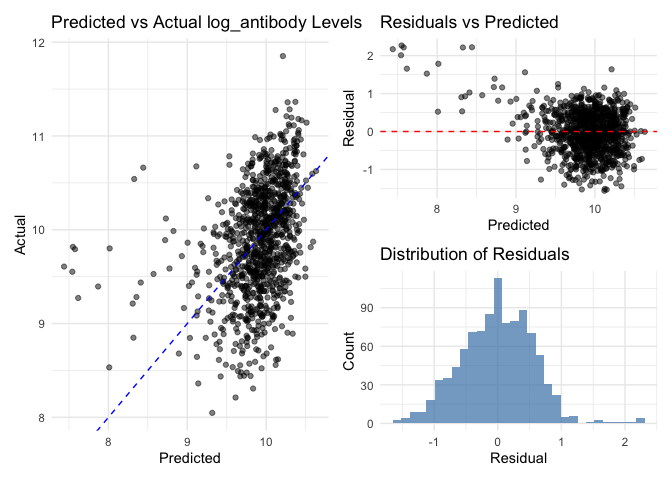
\includegraphics{DS2_Midterm_files/figure-latex/dx-plots-1.pdf}
\caption{Diagnostic Plots for Prediction Model on dat2}
\end{figure}

\textless\textless\textless\textless\textless\textless\textless{} HEAD
The prediction model's robustness and generalizability is mostly
acceptable for \textbf{dat2}. Prediction accuracy was determined by the
mean squared error (MSE) at 0.325 showing a low average on unseen data.
The prediction model shows model stability with generalized
cross-validation (GCV) score of 0.279. Looking at @ref(fig:dx-plots) we
evaluate Predicted vs Actual log\_antibody Levels, Residuals vs
Predicted, and the Distribution of Residuals. Predictions are mostly
aligned with the observed values especially in the 9.5-10.5 predicted
range. There is mild under-prediction below value 9, which indicates
that the model may tend to underestimate lower antibody levels but
perform well in the 9.5-10.5 predicted range. The predicted vs residual
plot shows residuals mostly centered and near 0, suggesting that there
is no significant bias in the model's predictions. Right-skewness can be
observed in the predicted vs residual plots, which could suggest some
non-linearity. The distribution of residuals looks approximately normal
and does not have extreme outliers or multi-modality. ======= The
prediction model's robustness and generalizability is mostly acceptable
for \textbf{dat2}. Prediction accuracy was determined by the mean
squared error (MSE) at 0.325 showing a low average on unseen data. The
prediction model shows model stability with generalized cross-validation
(GCV) score of 0.279. Looking at @ref(fig:dx-plots) we evaluate
Predicted vs Actual log\_antibody Levels, Residuals vs Predicted, and
the Distribution of Residuals. Predictions are mostly aligned with the
observed values especially in the 9.5-10.5 predicted range. There is
mild under-prediction below value 9, which indicates that the model may
tend to underestimate lower antibody levels but perform well in the
9.5-10.5 predicted range. The predicted vs residual plot shows residuals
mostly centered and near 0. Right-skewness can be observed in the
predicted vs residual plots, which could suggest some non-linearity. The
distribution of residuals looks approximately normal and does not have
extreme outliers or multi-modality.
\textgreater\textgreater\textgreater\textgreater\textgreater\textgreater\textgreater{}
f5e371ff37c9e841cbcaba1343c15e0de86916ee

\end{document}
